\newpage
\section{Example 3: Gap detection: determining the Just Noticeable Difference}

\todo{example needs modifications, corrector and choices = outdated? modified own version to create new figure }

\subsection{General description of the experiment}
See \filename{examples/manual/gapdetection.apx}. This is an
example of a gap detection task: two stimuli are presented to the
listener in random order, a stationary noise and an interrupted
noise. During the presentation the intervals are highlighted. The
subject's task is to indicate the interval with the
interruption(figure~\ref{fig:gapdetection}). Feedback is provided
(thumb up, thumb down) and the minimal detectable gap is
determined by means of an adaptive procedure (here 2-down, 1-up).
Stimuli (wave files) are generated off line. This example only
includes 5 wave files. Usually many more are generated. The
results are written to a text file.


\begin{figure}
 \centering
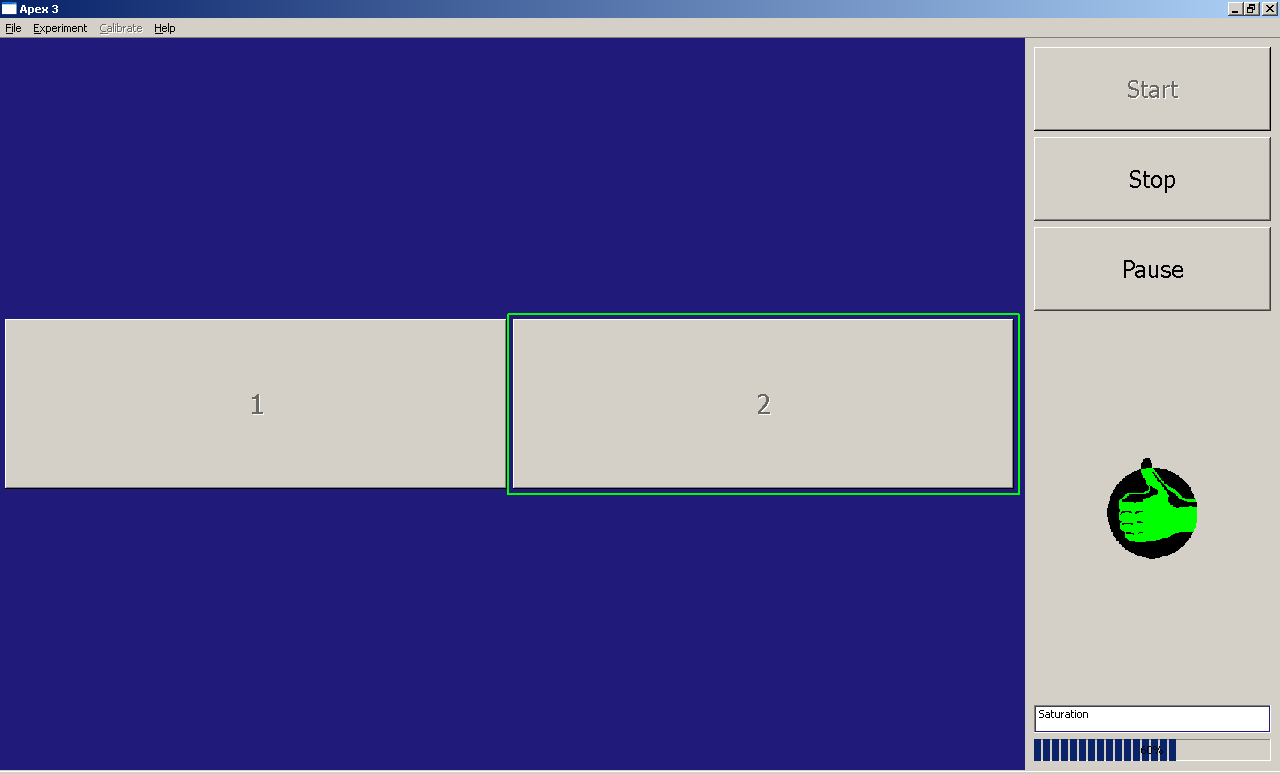
\includegraphics[width=\textwidth]{example3gapdetection.png}
 \caption{Example of adaptive gap detection experiment}
 \label{fig:gapdetection}
\end{figure}

\subsection{Conceptual}
The experiment as described in the previous paragraph should first
be translated to concepts understood by \apex. The main concepts
used here are \textbf{procedure}, \textbf{screens},
\textbf{datablocks} and \textbf{stimuli}.

For each wave file (noise with or without a gap) a \element
{datablocks} is defined, and for each datablock a \element
{stimulus} is defined. In this example there are 5 wave files,
with gap sizes ranging between 1 and 5 ms. Their IDs are
\id{g5ms}, \id{g4ms}, \id{g3ms},\id{g2ms} and \id{g1ms}. In an
adaptive procedure either a fixed or variable parameter is
defined. In this example a fixed parameter is used, i.e. the gap
size in the stimulus. The wave files with different gap sizes are
stored on disk, and are assigned a certain gap value. This gap
value is used to determine the gap threshold. Also, a \element
{screen} is defined that shows the two response intervals
indicating ``1'' and ``2''.

To indicate the order in which the stimuli should be presented a
\element {procedure} is defined. An adaptive procedure is defined
containing 1 \element {trial} with five variable stimuli (with
gap) and the standard stimulus without the gap. Recall that a
\element {trial} is the combination of a \element {screen} (always
the same in this example), a stimulus and a correct answer. The
standard and stimuli occur randomly in one of both intervals.

Now only the output logic remains to be defined. The idea is to
present the standard and a variable stimulus after each other, and
the stimulus to be presented depends on the response of the
subject. Filters are not used since the signals are not changed.

In the following sections each of the elements of the XML file
necessary to implement the latter concepts will be described in
detail.

\subsection{Detailed description of various elements}

\todo{modifications: to check, corrector?}
\begin{lstlisting} 
<procedure xsi:type="apex:adaptiveProcedure">
   <parameters>
     <presentations>1</presentations>
     <order>sequential</order>
     <intervals count="2">
	<interval number="1" element="button1"/>
	<interval number="2" element="button2"/>
	</intervals>
     <pause_between_stimuli>1000</pause_between_stimuli>
     <nUp>1</nUp>
     <nDown>2</nDown>
     <adapt_parameter>gap</adapt_parameter>
     <start_value>5</start_value>
     <stop_after_type>reversals</stop_after_type>
     <stop_after>5</stop_after>
     <min_value>0</min_value>
     <max_value>5</max_value>
     <larger_is_easier>true</larger_is_easier>
     <stepsizes>
       <change_after>reversals</change_after>
       <stepsize  begin="0" size="2"/>
       <stepsize begin="2" size="1"/>
     </stepsizes>
  </parameters>

  <trials>
    <trial id="trial1" >
     <screen id="screen1" />
     <stimulus id="stimulus1" />
     <stimulus id="stimulus2"/>
     <stimulus id="stimulus3"/>
     <stimulus id="stimulus4"/>
     <stimulus id="stimulus5"/>
     <standard id="standard"/>
    </trial>
  </trials>
</procedure>
\end{lstlisting}


\element{procedure} The attribute
\xml{xsi:type="adaptiveProcedureType"} refers to a procedure in which a parameter is changed according to
the response of the subject. In this example 1 trial is defined
with different stimuli from which the adaptive procedure chooses.

\begin{itemize}
\item \element{parameters} defines the behavior of the procedure
(eg., nr of presentations, order of presentation, response
strategy).

\begin{itemize}
\item \element{presentation} every trial is presented once.

\item \element{order} applies to the order of the trials. Since there is only 1
\element{trial}, it does not matter here wether the order is
specified as \element{sequential} or \element{random}.

\item \element{corrector} the corrector checks whether the
response is correct or not. In this example the number of choices
in \element{procedure} was 2. This means that \element{procedure}
will present the target stimulus in either interval 1 or 2.
\element{procedure} informs \element{corrector} about the correct
interval. \element{Corrector} also receives the clicked button from the
screen and looks up the corresponding number in the
\element{interval} element above and compares it with the number it
received from \element{procedure}. \todo{check}

\item \element{alternatives} number of alternatives to choose from
(here: 2 intervals) and the IDs of the buttons (defined under \element{screens} they correspond to.

\item \element{pause_between_stimuli} a pause of 1000 ms will be
introduced between successive wave files;

\item \element{nUp} number of items after incorrect trials to
increase the gap

\item \element{nDown} number of items after correct trials to
decrease the gap

\item \element{min_value} the gap size cannot be smaller than 0.

 \item \element{max_value} the gap size cannot be larger than 5

\item \element{adapt_parameter} the parameter to change, here the
``gap'', see also \element{fixed_parameters}

\item \element{start_value} the gap at which to start, here 5, see
under \element{stimulus}

\item \element{stop_after_type} reversals (it can also stop after
a number of presentations or trials)

\item \element{stop_after} number of reversals after which the
procedure is stopped

\item \element{rev_for_mean} the number of reversals that are used
for the average threshold

\item \element{larger_is_easier} here \xml{true} (the smaller the
gap, the more difficult the task)

\item \element{stepsizes} the stepsize

\end{itemize}

\begin{itemize}
\item\element{change_after} the \element{stepsize} is changed
after a specified number of reversals. In this example a stimulus
is skipped until the second reversal (start at 5, then 3, etc).
Thereafter no stimulus is skipped.

\end{itemize}

\item \element{trials} only 1 trial is defined

\begin{itemize}

\item \element{trial} the ID of the trial

\item\element{screen} the ID of the screen

\item \element{stimulus} the ID of the stimulus

\item \element{standard} the ID of the standard

\end{itemize}
\end{itemize}

\index{parameters}

\index{presentation}

\index{order}

\index{corrector}

\index{alternatives}

\index{pause between stimuli}

\index{nUp}

\index{nDown}

\index{adapt parameter}

\index{start value}

\index{stop after type}

\index{min value}

\index{max value}

\index{larger is easier}

\index{stepsize}

\index{trials}

\index{screen}

\index{stimulus}

\index{standard}



\begin{lstlisting}
<screens>
  <reinforcement>
    <progressbar>true</progressbar>
    <feedback length="300">true</feedback>
    <showcurrent>true</showcurrent>
  </reinforcement>

  <screen id="screen1" >
    <gridLayout height="1" width="2" id="main_layout">
      <button x="1" y="1" id="button1" >
       <text>1</text>
      </button>
      <button x="2" y="1" id="button2" >
       <text>2</text>
      </button>
    </gridLayout>
  <buttongroup id="buttongroup1">
     <button id="button1"/>
     <button id="button2"/>
  </buttongroup>
    <default_answer_element>buttongroup1</default_answer_element>
 </screen>
</screens>
\end{lstlisting}

\begin{itemize}
\item \element{screens} contains several screen elements that can
be referred to elsewhere in the experiment file (e.g. in
\element{procedure} above).


\item \element{reinforcement} includes elements on progress and
feedback

\begin{itemize}

\item \element{progressbar} if \xml {true} a progress bar will be
displayed in the right hand bottom corner of the screen. The
progress bar can indicate the percentage of trials that have been done or it
shows when a reversal occurs in an adaptive procedure. In the
latter case the progress bar will increase at every reversal while
the number of trials varies.

\item \element{feedback length} duration of the time after
response (in msec) that \apex waits before presenting the next
trial. During this interval feedback can be displayed.

\item \element{showcurrent} if \xml{true} the interval is highlighted while a
signal is presented.
\end{itemize}

\item \element{screen} each screen has an ID by which it can be
referred to elsewhere in the experiment. In this example the
screen displays two intervals.

\begin{itemize}


\item \element{gridlayout}places elements in an irregular grid.
The screen is divided into sections according to the values. In
this example there is an equal number of rows (x) and columns (y).

Gridlayout defines a group of screen elements (those that are
displayed on the screen).

\begin{itemize}
\item \element{button} for each interval a button is specified;
this button (interval) displays a number on the screen

\item \element{text} the left interval denotes ``1'', the right
one denotes ``2''.

\end{itemize}

\item \element{buttongroup} defines a group of screen elements
(those that are displayed on the screen). As many elements can be
defined in a screen, \apex has no way to know which element
contains the subject's response. Therefore, in
\element{default_answer_element} the element is designated that
contains the subject's response. In the case of screen elements
that are clicked in order to respond, the example is further
complicated by the fact that we cannot specify just one of the
elements (one button, one picture), but that the response rather comes
from a group of elements. This is when a \element{buttongroup} can
be used to group together different screen elements.

\end{itemize}
\end{itemize}



\index{screens}

\index{reinforcement}

\index{progressbar}

\index{feedback length}

\index{showcurrent}

\index{screen}

\index{gridlayout}

\index{button}

\index{text}

\index{buttongroup}

\index{default answer element}

\begin{lstlisting}
<datablocks>
  <uri_prefix>Gapfiles</uri_prefix>
    <datablock id="g5ms" >
      <device>wavdevice</device>
      <uri>g5.wav</uri>
    </datablock>

    <datablock id="g4ms" >
      <device>wavdevice</device>
      <uri>g4.wav</uri>
    </datablock>

    <datablock id="g3ms"  >
      <device>wavdevice</device>
      <uri>g3.wav</uri>
    </datablock>

    <datablock id="g2ms" >
      <device>wavdevice</device>
      <uri>g2.wav</uri>
    </datablock>

    <datablock id="g1ms"  >
      <device>wavdevice</device>
      <uri>g1.wav</uri>
    </datablock>

    <datablock id="datablockref">
      <device>wavdevice</device>
      <uri>ref500.wav</uri>
    </datablock>
  </datablocks>
\end{lstlisting}


\element{datablocks} contains a list of \element{datablock}
elements and a prefix.

\begin{itemize}
\item \element{uri_prefix}: a relative path is specified here.
Since \apex knows the location of the experiment file, only the
folder containing the wave files and pictures must be specified.



\item \element{datablock} for each wave file a unique datablock is
defined by an ID. The standard signal (uninterrupted noise) must
also be specified here.

\item \element{device} each datablock includes the audio device to
which the signal is routed

\item \element{uri} since the path is defined in
\element{uri_prefix} it is not necessary to specify the entire
path again

\index{datablocks} \index{uri prefix} \index{datablock}
\index{device} \index{uri}

\end{itemize}
\begin{lstlisting}
<devices>
 <device id="wavdevice" xsi:type="apex:wavDeviceType">
 <driver>portaudio</driver>
 <card>default</card>
 <channels>2</channels>
 <gain>0</gain>
 <samplerate>44100</samplerate>
 </device>
</devices>
\end{lstlisting}


\element{devices} all devices defined in the experiment file are
grouped in the \element{devices}. Only 1 \element{device} is used
in this example. The ID is set to soundcard. As an ID is unique
for an entire experiment file, it can be used later on to refer to
this device.

\begin{itemize}
\item \element{device} the \xml{xsi:type="apex:wavDeviceType"}
attribute tells \apex that a sound card is used. The experiment
only starts if all devices can be opened.

\item \element{driver} specifies the software driver to be used
for sound output. If unsure, set it to \xml{portaudio}.

\item \element{card} specifies the name of the sound card to be
used. The system default card can be used by specifying
\xml{default} as a card name. Other card names can be defined in
ApexConfig.

\item \element{channels} 2 channels are specified here, because
the signal is stereo.

\item \element{samplerate} the sampling frequency of the wave
files. Not all sampling rates are supported by all devices, and
some drivers automatically convert the sampling rate. Check your
sound card documentation. The sample rate of the sound card should
correspond to the sampling rates of all datablocks used with it.

\end{itemize}

\index{devices}

\index{driver}

\index{card}

\index{channels}

\index{gain}

\index{samplerate}


\begin{lstlisting}
<stimuli>
   <fixed_parameters>
     <parameter id="gap"/>
   </fixed_parameters>

   <stimulus id="stimulus1" >
     <description>noisewithgap1</description>
     <datablocks>
       <datablock id="g5ms" />
     </datablocks>
     <fixedParameters>
       <parameter id="gap">5</parameter>
     </fixedParameters>
   </stimulus>

   <stimulus id="stimulus2" >
     <description>noisewithgap2</description>
     <datablocks>
       <datablock id="g4ms" />
     </datablocks>
       <fixedParameters>
        <parameter id="gap">4</parameter>
     </fixedParameters>
   </stimulus>

   <stimulus id="stimulus3" >
     <description>noisewithgap3</description>
     <datablocks>
       <datablock id="g3ms" />
     </datablocks>
      <fixedParameters>
       <parameter id="gap">3</parameter>
      </fixedParameters>
   </stimulus>

   <stimulus id="stimulus4" >
     <description>noisewithgap4</description>
     <datablocks>
       <datablock id="g2ms" />
     </datablocks>
       <fixedParameters>
        <parameter id="gap">2</parameter>
       </fixedParameters>
   </stimulus>

   <stimulus id="stimulus5" >
     <description>noisewithgap5</description>
     <datablocks>
       <datablock id="g1ms" />
     </datablocks>
       <fixedParameters>
         <parameter id="gap">1</parameter>
       </fixedParameters>
   </stimulus>

   <stimulus id="standard">
     <datablocks>
      <datablock id="datablockref"/>
     </datablocks>
       <fixedParameters>
        <parameter id="gap">0</parameter>
     </fixedParameters>
   </stimulus>
</stimuli>
\end{lstlisting}


\element{stimuli} defines the auditory events, e.g. noise with gap
and noise without gap.

\begin{itemize}

\item \element{fixedParameters}

\begin{itemize}
\item \element{parameter} the gap is a fixed parameter that is
identified by an ID
\end{itemize}

\item \element{stimulus} this element includes a description of
the (variable) stimulus

\begin{itemize}
\item \element{description}

\item \element{datablocks} the ID refers to the wave file corresponding to the datablock

\item \element{fixedParameter}
\begin{itemize}
\item \element{parameter} includes information on the size of the
variable gap
\end{itemize}

\end{itemize}
\end{itemize}


\index{stimuli}

\index{fixed parameters}

\index{stimulus}

\index{datablocks}

\index{parameter}

\index{standard}

\begin{lstlisting}
<connections>
   <connection>
     <from>
       <id>_ALL_</id>
       <channel>0</channel>
     </from>
     <to>
       <id>wavdevice</id>
       <channel>1</channel>
     </to>
   </connection>

 </connections>
\end{lstlisting}

\index{connections} \index{channel}

\begin{itemize}
\item \element{connections} defines how the different datablocks
and filters are routed to the output device. The ID \id{_ALL_}
stands for all the datablocks. In this example they are routed to
1 channel of the wavdevice.
\end{itemize}

A visual representation of connections can be obtained by choosing
``Show stimulus connections'' under ``Experiment''in the main
\apex menu (top left menu bar).


\begin{lstlisting}
<results>
  <page>apex:resultsviewer.html</page>
  <resultparameters>
   <parameter name="reversals for mean">3</parameter>
  </resultparameters>
  <showduringexperiment>false</showduringexperiment>
  <showafterexperiment>true</showafterexperiment>
  <saveprocessedresults>true</saveprocessedresults>
 </results>
\end{lstlisting}

\element{results} Even if \element{results} is not specified in
the experiment file \apex will save a results file in XML. The results file
will display the correct answers, the reversals, the entire
sequence of responses, and the average threshold based on the
number of reversals and the magnitude of the corresponding gap
parameter specified in the experiment file.

\todo{new part, to check!}
\begin{itemize} 
\item \element{page} URL of the html page to show in the results window. The page should have the appropriate java script methods embedded. More example pages can be found in the \apex resultsviewer folder.
\item \element{resultparameters} Parameters to be passed to the results page. Each parameter will be set in hash params. \todo{perhaps some moren explanation on what this can be and why it is empty here?}
\item \element{showduringexperiment} If \xml{true}, an extra window will be created which will show the results of the current experiment while the experiment is being executed. Javascript embedded in the page will be executed upon each new trial.
\item \element{showafterexperiment} If \xml{true}, when the experiment is finished, a dialog box will appear querying whether results should be shown. If the answer is affirmative, a new window will be opened and the results will be shown after javascript processing.
\item \element{saveprocessedresults} If \xml{true} the
experimenter will be asked whether the processed results must be
appended to the results file. This will only work if the results are successfully saved to disk and your javascript code supports this transformation.
\end{itemize}

\index{results} \index{page} \index{resultparameters} \index{showduringexperiment} \index{showafterexperiment} \index{saveprocessedresults}



\begin{lstlisting}
 <general>
  <exitafter>true</exitafter>
 </general>
\end{lstlisting}

\element{general} defines some general parameters.

\begin{itemize}
\item \element{exitafter} if \xml{true} \apex will close after the experiment has ended and results have been shown.
\end{itemize}
